%%%%%%%%%%%%%%%%%%%%%%%%%%%%%%%%%%%%%%%%%%%%%%%%%
\section[Calibration]{Calibration}
%------------------------------------------------
%++++++++++++++++++++++++++++++++++++++++++++++++
\subsection{Système de calibrage}
%++++++++++++++++++++++++++++++++++++++++++++++++

\begin{frame}
\frametitle{Les différents repères}

\begin{minipage}{0.48\textwidth}
    \centering
    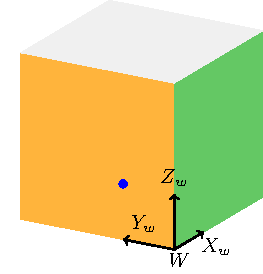
\includegraphics[width=\linewidth]{capture/cube_tikz.pdf}
    \vspace{0.5em}
    
    {\footnotesize\textbf{Représentation du cube (vue 3D)}}
\end{minipage}
\hfill
\begin{minipage}{0.48\textwidth}
    \centering
    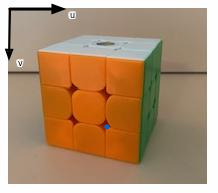
\includegraphics[width=\linewidth]{capture/cube_repere.png}
    \vspace{0.5em}

    {\footnotesize\textbf{Cube sur une image}}
\end{minipage}

\end{frame}

\begin{frame}{Modèle de projection — Matrice \( P \)}

\begin{itemize}
  \item<1-> On considère un point 3D \( M = (X, Y, Z) \)
  \item<2-> Il se projette sur un point image \( m = (u, v) \)
  \hyperlink{projection-appendix}{
    \beamerbutton{Compléments projections}
  }
  \item<3-> On cherche une relation linéaire homogène (pourquoi ?):
  \[
  \lambda
  \begin{bmatrix}
  u \cr v \cr 1
  \end{bmatrix}
  P
  =
  \begin{bmatrix}
  X \cr Y \cr Z \cr 1
  \end{bmatrix}
  \]

  \item<4-> \( P \) est une matrice \( 3 \times 4 \), avec 12 inconnues
  \item<5-> En développant les lignes :
  \[
  \lambda u = p_{11}X + p_{12}Y + p_{13}Z + p_{14}
  \]
  \[
  \lambda v = p_{21}X + p_{22}Y + p_{23}Z + p_{24}
  \]
  \[
  \lambda   = p_{31}X + p_{32}Y + p_{33}Z + p_{34}
  \]
\end{itemize}
\end{frame}

%------------------------

\begin{frame}{Équations sans \(\lambda\) et système matriciel}

\begin{itemize}
  \item<1-> Pour un point donné, on élimine \( \lambda \) :
  
  \[
  u (p_{31}X + p_{32}Y + p_{33}Z + p_{34}) = p_{11}X + p_{12}Y + p_{13}Z + p_{14}
  \]
  \[
  v (p_{31}X + p_{32}Y + p_{33}Z + p_{34}) = p_{21}X + p_{22}Y + p_{23}Z + p_{24}
  \]

  \vspace{0.5em}
   \item<2-> Cela donne un système homogène ...
   \[
   \scriptsize
   \begin{cases}
0= & p_{11} x_{C} +p_{12} y_{C}  +p_{13} z_{C} +p_{14} -p_{31} u x_{C} -p_{32} u  z_{C}  -p_{33} u  z_{C}  -p_{34} u \\
0= &  p_{21} x_{C}  +p_{22} y_{C}  +p_{23} z_{C}  +p_{24} -p_{31} v  x_{C}  -p_{32} v  z_{C}  -p_{33} v  z_{C}  -p_{34} v 
\end{cases}
   \]
  \item<3-> En faisant cela pour n points on obtient un système ...
\end{itemize}

\end{frame}


\begin{frame}{Équations sans \(\lambda\) et système matriciel}
  
\[
\resizebox{\textwidth}{!}{$
\left(
\begin{array}{cccccccccccc}
    x_{C}^{(1)} & y_{C}^{(1)} & z_{C}^{(1)} & 1 & 0 & 0 & 0 & 0 & -u^{( 1)} x{C}^{(1)} & -u^{( 1)}y{C}^{(1)} & -u^{( 1)}z_{C}^{(1)} & -u^{(1)}\\
0 & 0 & 0 & 0 & x_{C}^{( 1)} & y_{C}^{( 1)} & z_{C}^{( 1)} & 1 & -v^{( 1)} x_{C}^{( 1)} & -v^{( 1)} y_{C}^{( 1)} & -v^{( 1)} z_{C}^{( 1)} & -v^{( 1)}\\
\vdots  & \vdots  & \vdots  & \vdots  & \vdots  & \vdots  & \vdots  & \vdots  & \vdots  & \vdots  & \vdots  & \vdots \\
x_{C}^{( i)} & y_{C}^{( i)} & z_{C}^{( i)} & 1 & 0 & 0 & 0 & 0 & -u^{( i)} x_{C}^{( i)} & -u^{( i)} y_{C}^{( i)} & -u^{( i)} z_{C}^{( i)} & -u^{( i)}\\
0 & 0 & 0 & 0 & x_{C}^{( i)} & y_{C}^{( i)} & z_{C}^{( i)} & 1 & -v^{( i)} x_{C}^{( i)} & -v^{( i)} y_{C}^{( i)} & -v^{( i)} z_{C}^{( i)} & -v^{( i)}\\
\vdots  & \vdots  & \vdots  & \vdots  & \vdots  & \vdots  & \vdots  & \vdots  & \vdots  & \vdots  & \vdots  & \vdots \\
x_{C}^{( 6)} & y_{C}^{( 6)} & z_{C}^{( 6)} & 1 & 0 & 0 & 0 & 0 & -u^{( 6)} x_{C}^{( 6)} & -u^{( 6)} y_{C}^{( 6)} & -u^{( 6)} z_{C}^{( 6)} & -u^{( 6)}\\
0 & 0 & 0 & 0 & x_{C}^{( 6)} & y_{C}^{( 6)} & z_{C}^{( 6)} & 1 & -v^{( 6)} x_{C}^{( 6)} & -v^{( 6)} y_{C}^{( 6)} & -v^{( 6)} z_{C}^{( 6)} & -v^{( 6)}
\end{array}
\right)
\begin{pmatrix}
p_{11}\\
p_{12}\\
p_{13}\\
p_{14}\\
p_{21}\\
p_{22}\\
p_{23}\\
p_{24}\\
p_{31}\\
p_{32}\\
p_{33}\\
p_{34}
\end{pmatrix} =\begin{pmatrix}
0\\
0\\
0\\
0\\
0\\
0\\
0\\
0\\
0\\
0\\
0\\
0
\end{pmatrix}
$}
\]
\end{frame}

\subsection{En pratiques}


\begin{frame}{Calibration}
  \note{
    1. rubiks cube comme mire de calibrage, 
    permet d'identifier facilement les faces et d'y apposer un repère
    On créer des fichiers types avec les coordonnées des points pour chaque paire de faces et ils nous suffit de selectionner les points à la main pour calibrer }
 \centering
  \begin{minipage}{0.48\linewidth}
    \centering
    \begin{figure}
      \centering
      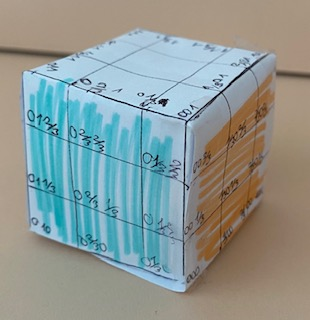
\includegraphics[width=0.7\linewidth]{capture/cube_calibrage.jpg}%
      \caption{Cube calibrage}
    \end{figure}
  \end{minipage}
  \hfill
  \begin{minipage}{0.48\linewidth}
    \centering
    \begin{figure}
      \centering
      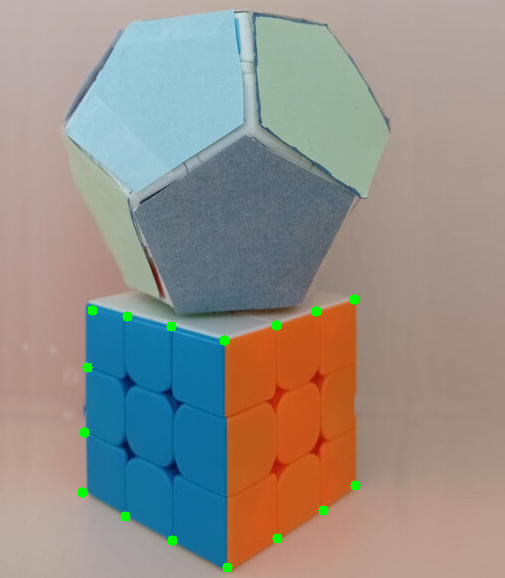
\includegraphics[width=0.8\linewidth]{capture/selection.png}%
      \caption{Selection des points}
    \end{figure}
  \end{minipage}
\end{frame}


\begin{frame}{Shooting photo : importance de la prise de vue}
  \note{
    au depart : on tourne autour/ faire tourner rubiks 
    fond unis mieux pour la Calibration
    face recouverte de papier pour etre unis et limiter les points inutiles
  }
  \centering
  \begin{minipage}{0.48\linewidth}
    \centering
    \begin{figure}
      \centering
      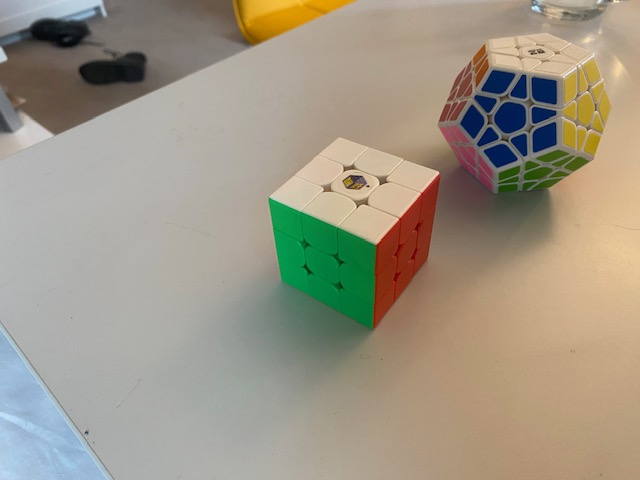
\includegraphics[width=0.48\linewidth]{capture/dodec0.jpg}%
      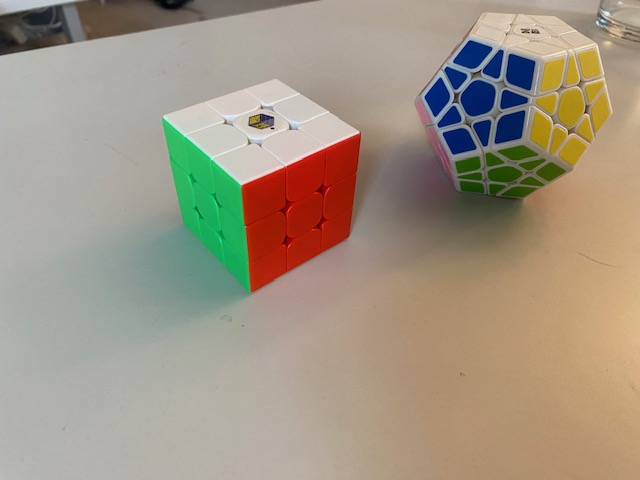
\includegraphics[width=0.48\linewidth]{capture/dodec1.jpg} \\
      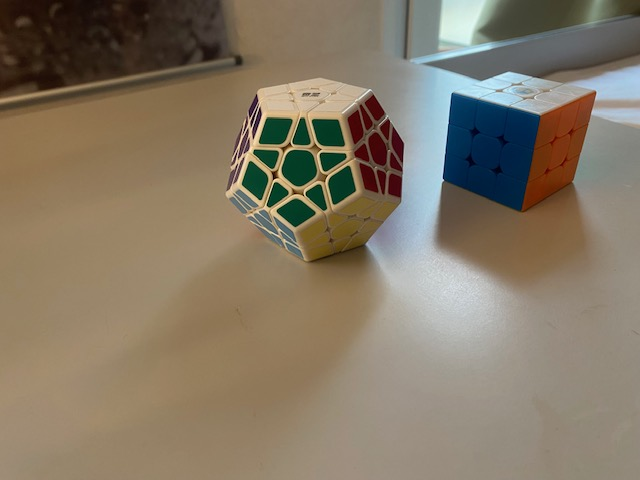
\includegraphics[width=0.48\linewidth]{capture/dodec2.jpg}%
      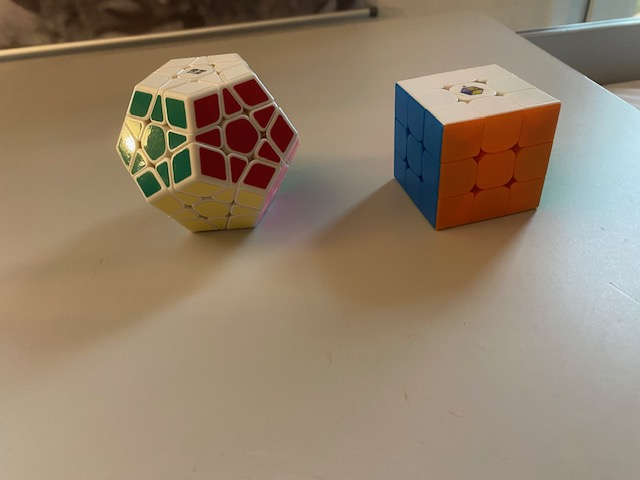
\includegraphics[width=0.48\linewidth]{capture/dodec3.jpg}
      {\footnotesize\textbf{Vues initiales}}
    \end{figure}
  \end{minipage}
  \hfill
  \begin{minipage}{0.48\linewidth}
    \centering
    \begin{figure}
      \centering
      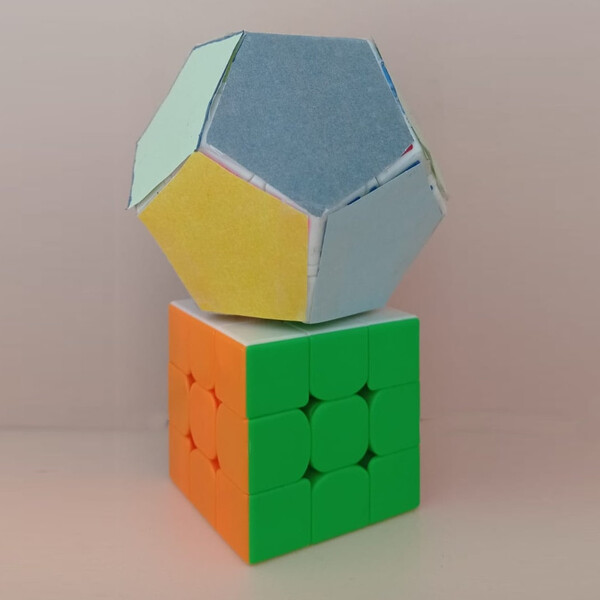
\includegraphics[width=0.48\linewidth]{capture/dodecf0.jpg}%
      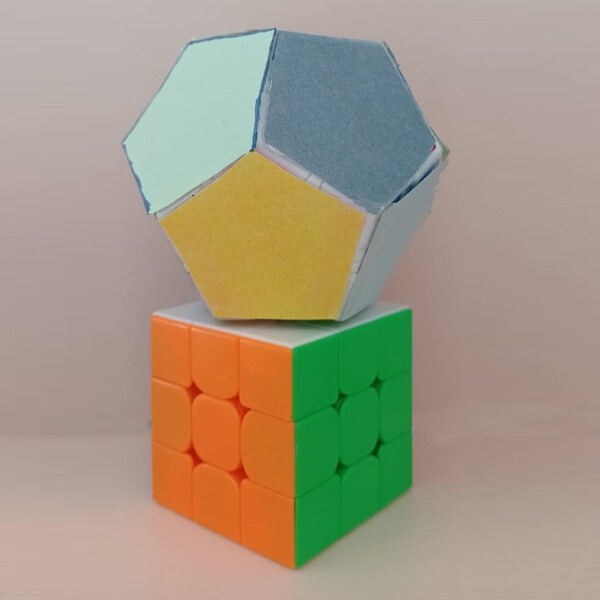
\includegraphics[width=0.48\linewidth]{capture/dodecf1.jpg} \\
      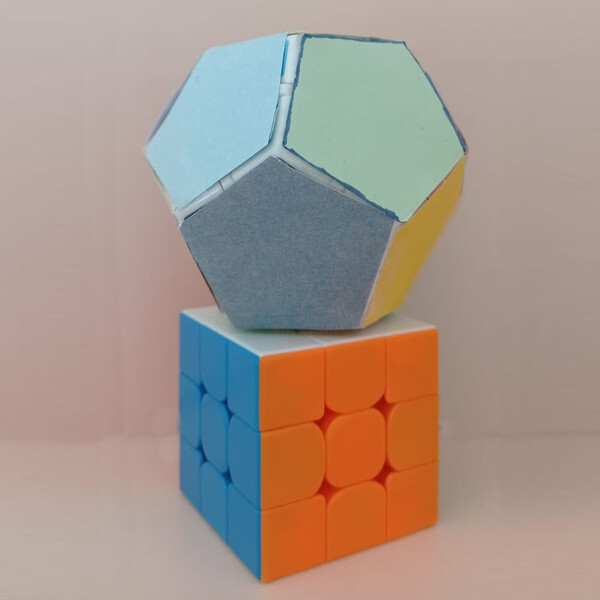
\includegraphics[width=0.48\linewidth]{capture/dodecf2.jpg}%
      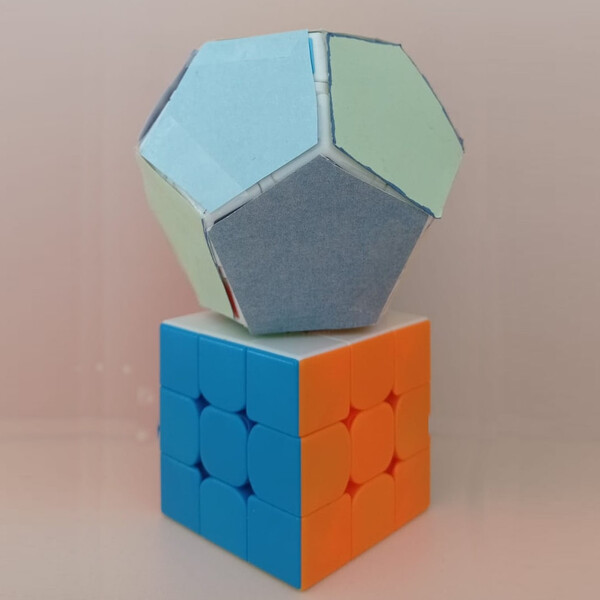
\includegraphics[width=0.48\linewidth]{capture/dodecf3.jpg}
      {\footnotesize\textbf{Vues améliorées}}
    \end{figure}
  \end{minipage}
\end{frame}